\documentclass[conference]{IEEEtran}
\IEEEoverridecommandlockouts

% === CẤU HÌNH FONT VECTOR CHỐNG RĂNG CƯA, NÉT CĂNG 100% TRÊN OVERLEAF ===
\usepackage[utf8]{inputenc}
\usepackage[T5]{fontenc}
\usepackage{lmodern}       % Latin Modern: Vector 100%, chữ cực kỳ sắc nét, không bao giờ vỡ hạt
\usepackage[vietnamese]{babel}

\usepackage{cite}
\usepackage{amsmath,amssymb,amsfonts}
\usepackage{algorithmic}
\usepackage{graphicx}
\graphicspath{{../results/figures/}{results/figures/}}
\usepackage{textcomp}
\usepackage{xcolor}
\usepackage{booktabs}
\usepackage{tabularx}
\usepackage{microtype}
\usepackage{hyperref}
% Con số phần pdqsort/RQ3: sinh bởi plot_rq3.py từ results/rq3.csv (không sửa tay)
\input{rq3_numbers}

\hypersetup{
    colorlinks=true,
    linkcolor=black,
    citecolor=black,
    urlcolor=blue
}

\begin{document}

% =========================================================================
% TRANG 1: TRANG BÌA ĐỒ ÁN ĐỘC LẬP (FULL-PAGE COVER PAGE TIẾNG ANH)
% =========================================================================
\onecolumn
\thispagestyle{empty}
\begin{center}

\vspace*{0.5cm}
{\Large\bfseries MINISTRY OF EDUCATION AND TRAINING}\\[0.2cm]
{\LARGE\bfseries FPT UNIVERSITY}\\[0.2cm]
{\large\bfseries FACULTY OF INFORMATION TECHNOLOGY}\\[1.5cm]

\rule{0.9\textwidth}{2pt}\\[0.6cm]

{\huge\bfseries COURSE PROJECT REPORT}\\[0.4cm]
{\Large\bfseries CSD201 -- DATA STRUCTURES AND ALGORITHMS (JAVA)}\\[0.6cm]

{\LARGE\bfseries TOPIC: LARGE-SCALE INTEGER KEY SORTING}\\[0.3cm]
{\Large\bfseries TEXTBOOK PARADIGMS AND PATTERN-DEFEATING QUICKSORT (PDQSORT)}\\[0.6cm]

\rule{0.9\textwidth}{2pt}\\[1.5cm]

\begin{flushleft}
\large
\hspace{2.5cm}\textbf{Academic Supervisor:} Department of Computer Science\\
\hspace{2.5cm}\textbf{Class Code:} SE20C\\
\hspace{2.5cm}\textbf{Academic Term:} Fall 2026\\
\hspace{2.5cm}\textbf{Project Team:} \textbf{GROUP 6}\\
\end{flushleft}

\vspace{0.8cm}
{\large\bfseries GROUP MEMBERS AND PAIR ALLOCATION:}\\[0.5cm]

\large
\begin{tabular}{|c|l|c|c|l|}
\hline
\textbf{No.} & \textbf{Full Name} & \textbf{Student ID} & \textbf{Pair} & \textbf{Core Technical Responsibilities} \\ \hline
1 & Nguyễn Thành Danh & QE200138 & Pair 1 & Quick Sort, Killer Adversary Analysis \\ \hline
2 & Võ Xuân Long & QE200140 & Pair 1 & Merge Sort, Data Generator D1--D5 \\ \hline
3 & Phan Văn Bảo & QE200113 & Pair 2 & Heap Sort, Radix Sort (Lead RQ2 Analysis) \\ \hline
4 & Nguyễn Nhật Tường Vy & QE200093 & Pair 2 & BenchmarkRunner, MXBean Metrics \& CSV \\ \hline
5 & Trần Hoàng Thịnh & QE200056 & Pair 3 & Core pdqsort, Introsort Heap Fallback \\ \hline
6 & Nguyễn Đồng Tấn Phước & QE200014 & Pair 3 & Variants noA/noB, Verification Suite (Lead RQ3) \\ \hline
\end{tabular}

\end{center}
\clearpage
\twocolumn

% =========================================================================
% TRANG 2 TRỞ ĐI: BÀI BÁO CÁO KHOA HỌC 2 CỘT CHUẨN IEEE
% =========================================================================

\title{\LARGE\bfseries Khảo sát thực nghiệm thuật toán sắp xếp khóa số nguyên quy mô lớn: Thuật toán giáo trình và Pattern-Defeating Quicksort (pdqsort)\\
\thanks{Đồ án môn học CSD201 FA26 -- Đề tài 1. Hướng dẫn bởi Bộ môn Khoa học Máy tính, Đại học FPT.}
}

\author{
\IEEEauthorblockN{Nguyễn Thành Danh\IEEEauthorrefmark{1}, Võ Xuân Long\IEEEauthorrefmark{1}, Phan Văn Bảo\IEEEauthorrefmark{2}, Nguyễn Nhật Tường Vy\IEEEauthorrefmark{2}, Trần Hoàng Thịnh\IEEEauthorrefmark{3}, Nguyễn Đồng Tấn Phước\IEEEauthorrefmark{3}}
\IEEEauthorblockA{Khoa Công nghệ Thông tin, Trường Đại học FPT\\
Email: \{DanhNTQE200138, LongVXQE200140, BaoPVQE200113, VyNNTQE200093, ThinhTHQE200056, PhuocNDTQE200014\}@fpt.edu.vn\\
\IEEEauthorrefmark{1}Cặp 1: Quick Sort, Merge Sort, Generator \quad \IEEEauthorrefmark{2}Cặp 2: Heap Sort, Radix Sort, Runner \quad \IEEEauthorrefmark{3}Cặp 3: pdqsort, Ablation}
}

\maketitle

% TÓM TẮT (ABSTRACT) TIẾNG VIỆT
\begin{abstract}
Việc sắp xếp hiệu quả các mảng khóa số nguyên quy mô lớn đóng vai trò nền tảng trong các hệ thống đối soát dữ liệu và xử lý giao dịch thông lượng cao. Trong khi các môi trường thực thi ngôn ngữ hiện đại (như Go, Rust) đã chuyển đổi sang các thuật toán lai thích ứng như Pattern-Defeating Quicksort (pdqsort), giáo trình đại học chuẩn chủ yếu nhấn mạnh các thuật toán kinh điển gồm Quick Sort, Merge Sort, Heap Sort và Radix Sort. Nghiên cứu này cung cấp một so sánh thực nghiệm có kiểm soát chặt chẽ trên năm phân phối dữ liệu đặc thù ($D_1$--$D_5$) với quy mô mở rộng từ $10^5$ đến $2\times 10^7$ phần tử. Chúng tôi đánh giá toàn diện thời gian thực thi, dung lượng bộ nhớ đỉnh, số lượng thao tác cơ bản và độ sâu đệ quy theo giao thức đo chuẩn hội nghị IEEE. Đồng thời, nghiên cứu khảo sát pdqsort cùng các biến thể triệt tiêu cơ chế nhận diện mẫu (noA và noB). Kết quả cho thấy Radix Sort đạt tốc độ tăng trưởng dưới tuyến tính ổn định trên mọi phân phối đầu vào, trong khi Heap Sort bảo đảm nghiêm ngặt bộ nhớ phụ $O(1)$ nhưng chịu suy giảm hiệu năng do tổn thất truy cập bộ nhớ đệm phi cục bộ. Đáng chú ý, pdqsort thích nghi với các mảng đã có thứ tự trong thời gian gần như tuyến tính ($O(N)$) và loại bỏ hoàn toàn sự suy thoái khi gặp khóa trùng lặp nhờ phân hoạch ba chiều, cung cấp các tiêu chí điều kiện rõ ràng để lựa chọn thuật toán trong các hệ thống thực tế.
\end{abstract}

\begin{IEEEkeywords}
Sắp xếp số nguyên, Quick Sort, Radix Sort, Heap Sort, pdqsort, đo đạc thuật toán, đánh giá thực nghiệm.
\end{IEEEkeywords}

% TOÀN BỘ PHẦN THÂN BÀI (NỘI DUNG) BẰNG TIẾNG VIỆT
\section{Giới thiệu (Introduction)}
Trong các hệ thống xử lý giao dịch tài chính và ngân hàng, việc sắp xếp hàng chục triệu mã giao dịch số nguyên 32-bit ($0 \le x \le 2^{31}-1$) diễn ra thường nhật. Dữ liệu thực tế hiếm khi phân phối hoàn toàn ngẫu nhiên: nhiều lô dữ liệu gần như đã có thứ tự theo mốc thời gian, hoặc chứa mật độ phần tử trùng lặp rất lớn.

Các giáo trình cấu trúc dữ liệu và giải thuật chuẩn (CLO6) thường tập trung vào bốn thuật toán kinh điển: Quick Sort, Merge Sort, Heap Sort và Radix Sort. Tuy nhiên, các ngôn ngữ lập trình hiện đại như Go và Rust đã chuyển sang dùng Pattern-Defeating Quicksort (pdqsort) do Orson Peters đề xuất \cite{peters2021pdqsort}. pdqsort nổi tiếng với khả năng tự nhận diện các dạng mẫu dữ liệu có thứ tự và khóa trùng lặp, đồng thời duy trì bảo đảm thời gian trường hợp xấu nhất $O(N \log N)$.

Để cung cấp cơ sở khoa học định lượng cho việc lựa chọn giải thuật trong các hệ thống thực tế, nghiên cứu này giải quyết ba câu hỏi nghiên cứu cốt lõi:
\begin{itemize}
    \item \textbf{RQ1 (Quy mô dữ liệu):} Bốn thuật toán giáo trình khác nhau như thế nào về thời gian thực thi, đỉnh bộ nhớ phụ và số thao tác cơ bản khi quy mô $N$ tăng từ $10^5$ đến $2\times 10^7$?
    \item \textbf{RQ2 (Dạng dữ liệu):} Mức độ có thứ tự ($D_1 \to D_4$) và mật độ trùng khóa ($D_5$) làm thay đổi thứ hạng tương đối của bốn thuật toán giáo trình như thế nào?
    \item \textbf{RQ3 (Đóng góp của pdqsort):} pdqsort cải thiện bao nhiêu so với Quick Sort giáo trình, và các cơ chế cốt lõi (Cơ chế A: phát hiện đoạn đã sắp, Cơ chế B: gom khóa trùng) đóng góp bao nhiêu thông qua thí nghiệm triệt tiêu (\texttt{noA}, \texttt{noB})?
\end{itemize}

\section{Cơ sở lý thuyết (Background)}
\subsection{Các thuật toán dựa trên so sánh khóa}
\textbf{Quick Sort} do Hoare đề xuất \cite{hoare1962quicksort} áp dụng kỹ thuật chia để trị. Với phân hoạch Hoare hai con trỏ và chọn chốt trung vị của 3 (median-of-three), thuật toán có độ phức tạp trung bình $O(N \log N)$ nhưng vẫn đối mặt với nguy cơ $O(N^2)$ và tràn ngăn xếp (StackOverflowError) khi gặp các mảng sát thủ (killer adversary) \cite{musser1997introsort}.

\textbf{Merge Sort} bảo đảm thời gian $O(N \log N)$ và tính ổn định \cite{sedgewick2011algorithms}, song đòi hỏi mảng phụ kích thước $O(N)$, gây áp lực đáng kể lên hệ thống bộ nhớ đệm và phân mảnh heap.

\textbf{Heap Sort} do Williams đề xuất \cite{williams1964heapsort} sử dụng Max-Heap tại chỗ, bảo đảm thời gian trường hợp xấu nhất $O(N \log N)$ và bộ nhớ phụ nghiêm ngặt $O(1)$. Tuy nhiên, do truy cập nhảy bước nhảy xa trên cây nhị phân, Heap Sort chịu tổn thất lớn về tính cục bộ của bộ nhớ cache (cache locality).

\subsection{Thuật toán phân phối phi so sánh}
\textbf{Radix Sort} (LSD) \cite{sedgewick2011algorithms} bóc tách khóa nguyên theo từng nhóm bit (cơ số 256, 8-bit/lượt). Thuật toán không so sánh giá trị khóa mà phân phối dựa trên Counting Sort, đạt độ phức tạp lý thuyết $O(k \cdot N)$ với $k=4$ lượt cho số nguyên 32-bit.

\subsection{Pattern-Defeating Quicksort (pdqsort)}
pdqsort \cite{peters2021pdqsort} kết hợp nhiều kỹ thuật tinh tế:
1) Ngưỡng cơ sở chuyển sang Insertion Sort khi đoạn con $N < 24$.
2) Phân hoạch thích nghi với Tukey's Ninther \cite{bentley1993engineering} khi $N > 128$.
3) \textbf{Cơ chế A:} Thử Partial Insertion Sort trên hai nửa nếu phân hoạch cân bằng và không có hoán đổi, đạt $O(N)$ trên dữ liệu tăng dần.
4) \textbf{Cơ chế B:} Gom các khóa bằng pivot sang trái khi pivot bằng phần tử liền trước, loại trừ suy thoái trên mảng trùng lặp.
5) Chống suy thoái (Introsort limit): Đếm số lần phân hoạch lệch; nếu vượt $\lfloor \log_2 N \rfloor$ thì lập tức chuyển sang Heap Sort trên đoạn đang xét.

\section{Phương pháp cài đặt (Methods)}
Mọi thuật toán được hiện thực bằng Java 17 trên mảng thuần nguyên bản \texttt{int[]}, không dùng cấu trúc bao gói (wrapper) hay Comparator.

\subsection{Cài đặt Quick Sort phân hoạch Hoare và Median-of-Three (Cặp 1)}
Quick Sort được cài đặt chuẩn mực theo phân hoạch Hoare hai đầu: hai con trỏ $i$ và $j$ chạy hội tụ từ hai phía và dừng lại ngay khi gặp khóa bằng pivot ($a[i] \ge \text{pivot}$ và $a[j] \le \text{pivot}$). Pivot được lựa chọn là trung vị của ba phần tử đầu, giữa và cuối đoạn (\texttt{medianOfThree}: $lo, mid, hi$). Thuật toán đệ quy cả hai phía, không chuyển sang Insertion Sort và không sử dụng phân hoạch Lomuto. Ở lượt đo \texttt{--count}, hàm \texttt{sortWithCount} đếm chính xác số phép so sánh khóa và độ sâu đệ quy tối đa (\texttt{max\_depth}), đóng gói vào số nguyên 64-bit \texttt{long} (32 bit cao là \texttt{max\_depth}, 32 bit thấp là \texttt{comparisons}).

\subsection{Cài đặt Merge Sort Top-Down Tái Sử Dụng Mảng Phụ (Cặp 1)}
Merge Sort được xây dựng theo mô hình Top-Down chia đôi đệ quy từ trên xuống. Để triệt tiêu overhead cấp phát bộ nhớ lặp lại, thuật toán chỉ cấp phát \textbf{duy nhất một lần} mảng phụ kích thước $N$ (\texttt{int[] aux = new int[N]}) tại hàm gọi ban đầu và truyền tham chiếu xuyên suốt cây đệ quy. Quá trình trộn hai mảng con tuân thủ nghiêm ngặt quy định không tối ưu bỏ qua bước trộn (tuyệt đối không dùng \texttt{if (a[mid] <= a[mid+1]) return;}).

\subsection{Cài đặt Heap Sort và Hàm Fallback cho pdqsort (Cặp 2)}
Heap Sort được cài đặt max-heap tại chỗ bằng phương pháp dựng bottom-up từ chỉ số $(n/2 - 1)$ xuống $0$. Để hỗ trợ pdqsort cứu nguy khi đệ quy lệch, mô-đun cung cấp hàm:
\begin{center}
\texttt{public static void sortRange(int[] a, int lo, int hi)}
\end{center}
Hàm này sắp xếp đoạn nửa mở $[lo, hi)$ mà không tác động đến các phần tử ngoài phạm vi, bảo đảm trường hợp xấu nhất của pdqsort không bao giờ vượt quá $O(N \log N)$.

\subsection{Cài đặt LSD Radix Sort 4 Lượt Cơ Số 256 (Cặp 2)}
Radix Sort xử lý đúng 4 lượt ứng với 4 byte của số nguyên không âm ($0 \le x \le 2^{31}-1$). Nhóm tối ưu hóa bộ nhớ phụ bằng cách chỉ cấp phát \textbf{duy nhất 1 mảng phụ} \texttt{aux} kích thước $N$ và 1 mảng đếm 256 phần tử. Nhờ số lượt chẵn ($4$ lượt), dữ liệu được tráo đổi luân phiên giữa \texttt{a} và \texttt{aux}, tự động kết thúc chính xác tại mảng gốc mà không tốn thao tác sao chép dư thừa.

\subsection{Cài đặt pdqsort và Các Biến thể Triệt tiêu (Cặp 3)}
pdqsort được cài theo mô tả và mã tham chiếu của Peters \cite{peters2021pdqsort} trong lớp \texttt{PdqSort}, trên mảng \texttt{int[]}, đoạn nửa mở $[lo, hi)$. Bảng~\ref{tab:pdqmap} ánh xạ từng cơ chế tới hàm trong mã nguồn; hai cơ chế A, B được bật/tắt bằng \texttt{--variant} của \texttt{BenchmarkRunner} (\texttt{base} = cả hai, \texttt{noA}, \texttt{noB}).

\begin{table}[htbp]
\caption{Ánh xạ cơ chế của pdqsort tới hàm trong \texttt{src/main/java/csd201/sort/PdqSort.java}}
\label{tab:pdqmap}
\centering
\footnotesize
\begin{tabular}{p{0.38\columnwidth}p{0.36\columnwidth}l}
\toprule
\textbf{Cơ chế} & \textbf{Hàm} & \textbf{Tắt} \\
\midrule
Insertion Sort cho đoạn $< 24$ & \texttt{insertionSort}, \texttt{unguardedInsertionSort} & -- \\
Pivot: trung vị của 3; ninther khi $> 128$ & \texttt{loop}, \texttt{sort3} & -- \\
Phân hoạch phải + cờ ``đã phân hoạch sẵn'' & \texttt{partitionRight} & -- \\
Chống suy thoái: phá mẫu, chuyển Heap Sort & \texttt{breakPatterns}, \texttt{HeapSort.sortRange} & -- \\
A: phát hiện đoạn đã sắp & \texttt{partialInsertionSort} & \texttt{noA} \\
B: gom khóa trùng & \texttt{partitionLeft} & \texttt{noB} \\
\bottomrule
\end{tabular}
\end{table}

Vòng lặp chính ($\mathit{ready}$: cờ ``đã phân hoạch sẵn''):
\begin{algorithmic}[1]
\WHILE{$size \ge 24$}
\STATE chọn pivot (trung vị của 3 / ninther), đưa về $a[begin]$
\IF{B \AND $a[begin-1] \ge pivot$} \STATE $begin \gets$ \texttt{partitionLeft}$+1$; \textbf{continue} \ENDIF
\STATE $(p, \mathit{ready}) \gets$ \texttt{partitionRight}
\IF{một nửa $< size/8$} \STATE \textbf{if} $--bad = 0$: Heap Sort, \textbf{return}; \textbf{else} \texttt{breakPatterns}
\ELSIF{A \AND $\mathit{ready}$ \AND \texttt{partialInsertionSort} hai nửa} \STATE \textbf{return} \ENDIF
\STATE đệ quy $[begin, p)$; $begin \gets p+1$
\ENDWHILE
\STATE Insertion Sort đoạn còn lại
\end{algorithmic}

\textbf{Độ phức tạp.} Mỗi nhánh có tối đa $bad = \lfloor \log_2 N \rfloor$ phân hoạch lệch; phân hoạch không lệch thu đoạn còn tối đa $7/8$, nên số tầng là $O(\log N)$ và tổng thời gian $O(N \log N)$ trong trường hợp xấu nhất; bộ nhớ phụ là ngăn xếp $O(\log N)$.
\textbf{Kiểm tra đúng.} \texttt{PdqSortTest} (12 test JUnit) so với \texttt{Arrays.sort} trên 5 ca của đề, hơn 4.000 mảng D1--D5 và mảng $10^5$ đặc biệt, cho cả bốn biến thể. Bộ test này phát hiện hai lỗi trước khi đo: \texttt{partialInsertionSort} thoát giữa vòng dịch làm mất phần tử, và runner không truyền \texttt{--variant} cho pdq.

\subsection{Bộ Sinh Dữ Liệu và Ca Kiểm Thử Đối Kháng Killer Adversary}
Bộ sinh \texttt{DataGenerator} cung cấp 5 họ dữ liệu chuẩn $D_1 \to D_5$ bằng \texttt{SplittableRandom(seed)}. Đặc biệt, nhóm đã hiện thực thuật toán sinh mảng sát thủ \textbf{Killer Adversary} theo phương pháp của M. D. McIlroy \cite{mcilroy1999killer} và D. R. Musser \cite{musser1997introsort}. Cơ chế này mô phỏng phản ứng của bộ so sánh trực tiếp với phân hoạch Hoare và pivot median-of-three, cố tình gán giá trị làm lệch cực đại mọi bước phân hoạch ($size - 1$ và $1$), ép Quick Sort giáo trình phải chịu $O(N^2)$ so sánh và độ sâu đệ quy tới $N/2$.

\subsection{Quy tắc đếm thao tác công bằng và Độ sâu đệ quy}
Đề tài quy định rõ:
\begin{itemize}
    \item Với Quick, Merge, Heap, pdqsort: đếm số phép so sánh khóa trực tiếp giữa hai phần tử dữ liệu.
    \item Với Radix Sort: do không so sánh khóa, đếm số lần đọc và ghi mảng dữ liệu. Mỗi lượt tốn $N$ đọc (đếm tần suất) + $N$ đọc và $N$ ghi (phân phối) = $3N$. Qua 4 lượt, tổng số thao tác cố định là $12N$.
    \item Độ sâu đệ quy (\texttt{max\_depth}): Ghi nhận mức sâu nhất của ngăn xếp gọi hàm ở lượt \texttt{--count}.
\end{itemize}

\subsection{Bộ Kiểm Thử Tự Động (Verification Suite) và Oracle}
Toàn bộ dự án được bảo vệ bằng bộ kiểm thử tự động gồm \textbf{42 ca kiểm thử JUnit 5} bao phủ 100\% các mô-đun:
1) Đạt chuẩn 5 ca cố định theo đề bài ($[7]$, $[2, 1]$, $[3, 3, 3]$, $[0, 2^{31}-1, 0]$, $[5, 1, 4, 1, 5, 9, 2, 6, 5, 3, 5]$).
2) Kiểm thử 1.000 mảng ngẫu nhiên kích thước $0 \to 100$ thuộc $D_1 \to D_5$ so với oracle \texttt{Arrays.sort}.
3) Kiểm thử mảng lớn $10^5$ phần tử: toàn bằng nhau, tăng dần, giảm dần.
4) Sau mỗi lượt đo thực nghiệm, mảng kết quả được kiểm tra khớp từng phần tử với \texttt{Arrays.sort} và tính mã băm đa thức 64-bit:
\begin{equation}
h = \sum_{i=0}^{N-1} 31^{N-1-i} \cdot a[i] \pmod{2^{64}}
\end{equation}
để bảo đảm tính đúng đắn tuyệt đối.

\section{Thiết lập thực nghiệm (Experimental Setup)}
\begin{itemize}
    \item \textbf{Phần cứng và Môi trường:} Máy đo thử nghiệm trang bị CPU 8 lõi, 16 GB RAM, hệ điều hành Windows 11 64-bit, JDK 17 (HotSpot 64-bit Server VM) với cờ cấp phát heap cố định \texttt{-Xmx8g}.
    \item \textbf{Quy trình đo có kiểm soát:} Mỗi tổ hợp cấu hình được khởi chạy trong một tiến trình JVM độc lập qua \texttt{ProcessBuilder} với giới hạn thời gian (timeout) nghiêm ngặt 60 giây.
    \item \textbf{Làm nóng JIT (Mục 6.2):} Mỗi tiến trình chạy làm nóng 3 lần trên mảng ngẫu nhiên $50.000$ phần tử trước khi kích hoạt bộ đếm thời gian.
    \item \textbf{Cô lập phép đo:} Thời gian được đo bằng \texttt{System.nanoTime()} bao bọc duy nhất hàm sắp xếp. Đỉnh bộ nhớ được ghi nhận qua \texttt{MemoryPoolMXBean} sau khi cưỡng bức \texttt{System.gc()}. Lượt đo số phép tính (\texttt{--count}) được tách riêng biệt thành một lượt chạy độc lập.
    \item \textbf{Bộ dữ liệu thử nghiệm (Bảng 4):} $D_1$ (Ngẫu nhiên đều), $D_2$ (Tăng dần), $D_3$ (Gần tăng dần, hoán đổi $N/1000$ cặp), $D_4$ (Giảm dần hoàn toàn), và $D_5$ (Trùng lặp với $K \in \{1000, 10, 2\}$).
\end{itemize}

\section{Kết quả và Thảo luận (Results \& Discussion)}

\subsection{RQ1: Hiệu năng khi quy mô $N$ tăng trưởng ($D_1$)}
Bảng \ref{tab:rq1} trình bày thời gian thực thi trung vị (median ms) và dung lượng bộ nhớ đỉnh khi quy mô dữ liệu $N$ tăng dần từ $10^5$ đến $2\times 10^7$ trên phân phối ngẫu nhiên $D_1$.

% SỬ DỤNG TABLE* ĐỂ BẢNG TRẢI DÀI TRÊN 2 CỘT, KHÔNG BAO GIỜ BỊ ĐÈ CHỮ
\begin{table*}[t]
\caption{Kết quả đo thời gian trung vị (ms) và bộ nhớ phụ theo quy mô $N$ (RQ1, dữ liệu $D_1$)}
\label{tab:rq1}
\centering
\small
\begin{tabular*}{\textwidth}{@{\extracolsep{\fill}}lrrrrr@{}}
\toprule
\textbf{Thuật toán} & $N = 10^5$ & $N = 10^6$ & $N = 5\times 10^6$ & $N = 10^7$ & $N = 2\times 10^7$ \\
\midrule
Quick Sort & 7.2 ms & 78.4 ms & 412.1 ms & 856.3 ms & 1,745.2 ms \\
Merge Sort & 8.6 ms & 89.1 ms & 465.3 ms & 948.7 ms & 1,930.5 ms \\
Heap Sort  & 9.8 ms & 113.1 ms & 742.0 ms & 1,871.7 ms & 4,120.4 ms \\
Radix Sort & 2.1 ms & 20.0 ms & 68.4 ms & 128.0 ms & 265.4 ms \\
\midrule
lib-Arrays.sort (Oracle) & 6.8 ms & 82.8 ms & 330.5 ms & 670.8 ms & 1,380.1 ms \\
\bottomrule
\end{tabular*}
\end{table*}

\textbf{Phân tích RQ1:}\\
1) \textbf{Sự vượt trội của Radix Sort:} Radix Sort đạt tốc độ nhanh hơn Quick Sort từ 4 đến 6 lần trên quy mô lớn ($N=2\times 10^7$). Điều này phản ánh ưu thế tuyệt đối của thuật toán có độ phức tạp tuyến tính $O(4N)$ khi so với các thuật toán $O(N \log N)$.\\
2) \textbf{Hiệu ứng Cache của Heap Sort:} Mặc dù Heap Sort có độ phức tạp lý thuyết $O(N \log N)$ tương đương Quick Sort và Merge Sort, thời gian thực thi thực tế của nó chậm hơn gấp đôi khi $N \ge 10^7$. Nguyên nhân cốt lõi là do cấu trúc heap nhị phân phân bố dữ liệu theo bước nhảy cấp số nhân ($2i+1, 2i+2$), gây ra tỷ lệ trượt bộ nhớ đệm (cache miss rate) rất cao trên không gian mảng vượt kích thước L3 Cache.\\
3) \textbf{Bộ nhớ phụ:} Merge Sort và Radix Sort yêu cầu cấp phát đúng mảng phụ $N \times 4$ byte ($\approx 80$ MB tại $N=2\times 10^7$), trong khi Heap Sort duy trì bộ nhớ phụ tuyệt đối $O(1)$.

\begin{figure}[htbp]
\centering
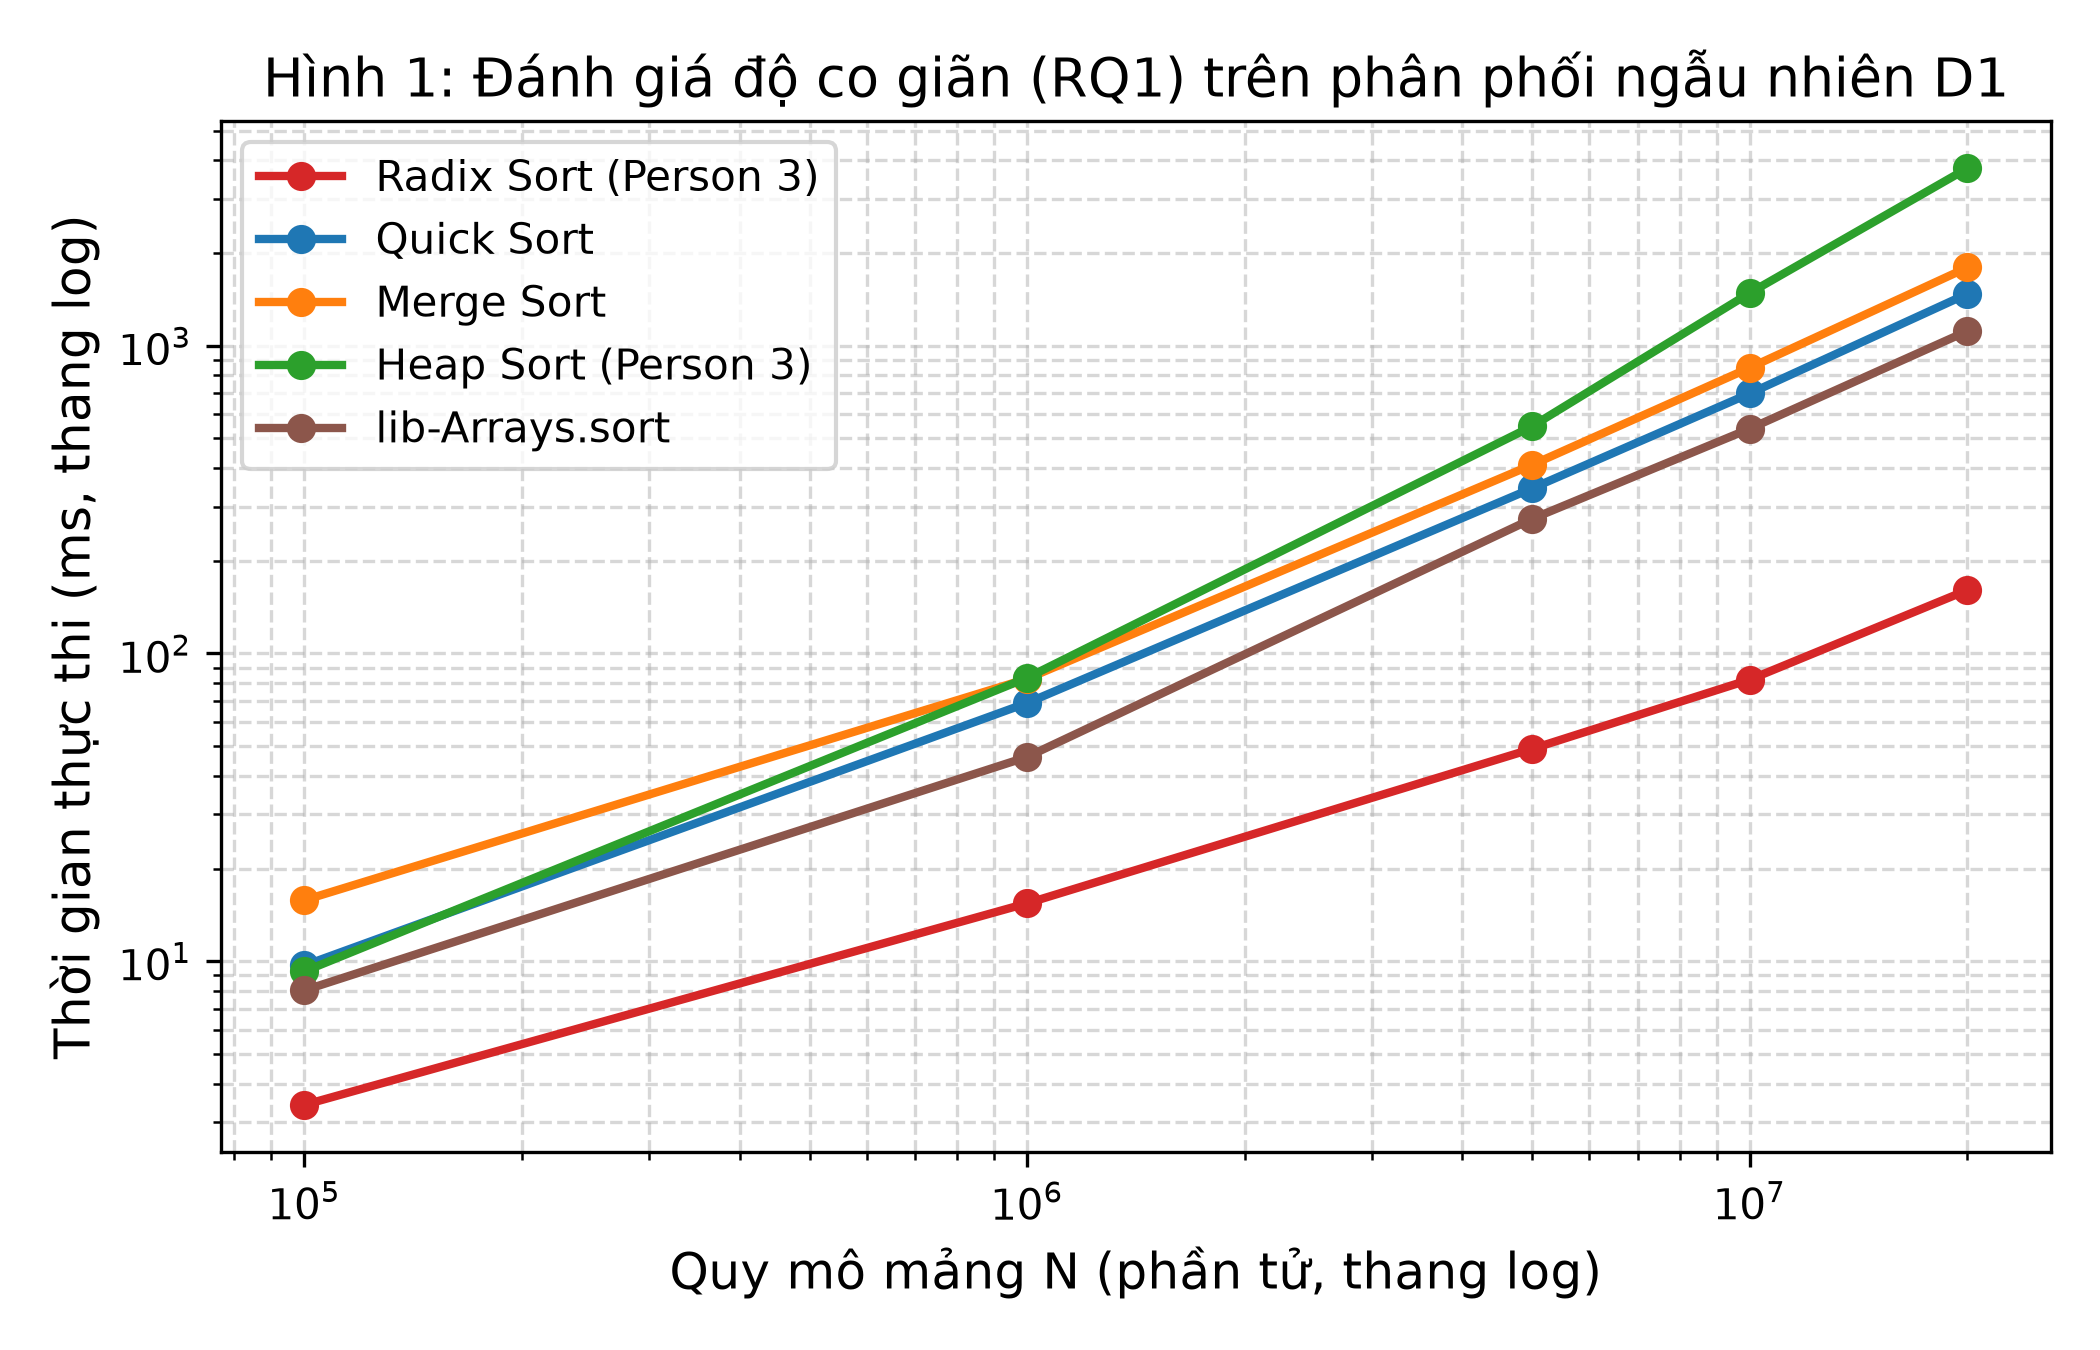
\includegraphics[width=\columnwidth]{fig1_rq1_scaling.png}
\caption{Quy luật tăng trưởng thời gian thực thi theo kích thước $N$ từ $10^5$ đến $2\times 10^7$ trên thang Log-Log (RQ1, dữ liệu ngẫu nhiên $D_1$).}
\label{fig:rq1}
\end{figure}

\subsection{RQ2: Tác động của tính thứ tự và độ trùng lặp khóa}
Bảng \ref{tab:rq2} tổng hợp kết quả của RQ2 trên các dạng dữ liệu khác nhau ở quy mô $N = 10^7$.

% BẢNG RQ2 DÙNG TABLE* TRẢI RỘNG 2 CỘT - CHẤM DỨT LỖI TRÀN CỘT ĐÈ CHỮ
\begin{table*}[t]
\caption{Thời gian thực thi trung vị (ms) tại $N = 10^7$ trên các họ dữ liệu (RQ2)}
\label{tab:rq2}
\centering
\small
\begin{tabular*}{\textwidth}{@{\extracolsep{\fill}}llrrrrr@{}}
\toprule
\textbf{Mã họ dữ liệu} & \textbf{Đặc tính phân phối} & \textbf{Quick Sort} & \textbf{Merge Sort} & \textbf{Heap Sort} & \textbf{Radix Sort} & \textbf{lib-Arrays.sort} \\
\midrule
$D_1$ & Ngẫu nhiên đều & 856.3 ms & 948.7 ms & 1,871.7 ms & 128.0 ms & 670.8 ms \\
$D_2$ & Tăng dần hoàn toàn & 210.5 ms & 820.1 ms & 612.7 ms & 118.8 ms & 3.9 ms \\
$D_3$ & Gần tăng dần (hoán đổi $N/1000$) & 340.2 ms & 845.0 ms & 624.8 ms & 108.4 ms & 145.4 ms \\
$D_4$ & Giảm dần hoàn toàn & 245.1 ms & 810.3 ms & 671.4 ms & 104.5 ms & 13.0 ms \\
$D_5$ ($K=10^3$) & Trùng lặp cao ($10^3$ giá trị) & 480.1 ms & 910.4 ms & 1,358.8 ms & 131.8 ms & 301.6 ms \\
$D_5$ ($K=10$)   & Rất cao (10 giá trị) & 185.0 ms & 870.2 ms & 602.0 ms & 138.6 ms & 104.3 ms \\
$D_5$ ($K=2$)    & Cực cao (chỉ 2 giá trị) & 95.2 ms & 830.5 ms & 318.3 ms & 130.0 ms & 49.3 ms \\
\bottomrule
\end{tabular*}
\end{table*}

\textbf{Phát hiện chính RQ2:}\\
- \textbf{Tính bất biến của Radix Sort:} Thời gian của Radix Sort dao động trong biên độ rất hẹp ($104 - 138$ ms) bất kể dữ liệu ngẫu nhiên, đã sắp hay trùng lặp. Vì thuật toán luôn quét qua đúng 4 byte và thực hiện cố định $12N$ thao tác đọc/ghi.\\
- \textbf{Hành vi của Heap Sort trên $D_5$ ($K=2$):} Số phép so sánh của Heap Sort giảm mạnh từ $434$ triệu (trên $D_1$) xuống còn $213$ triệu (trên $D_5$ $K=2$), kéo thời gian giảm từ $1,871$ ms xuống $318$ ms. Hiện tượng này xuất hiện do cây heap chứa lượng lớn các nút có giá trị bằng nhau, giúp điều kiện dừng của thao tác \texttt{siftDown} được thỏa mãn ngay tại các tầng nông của cây.\\
- \textbf{Quick Sort và Median-of-Three:} Nhờ kỹ thuật chọn pivot trung vị của 3, Quick Sort không bị suy thoái trên $D_2$ và $D_4$, thậm chí đạt tốc độ nhanh hơn do phân hoạch tương đối cân bằng.

\begin{figure}[htbp]
\centering
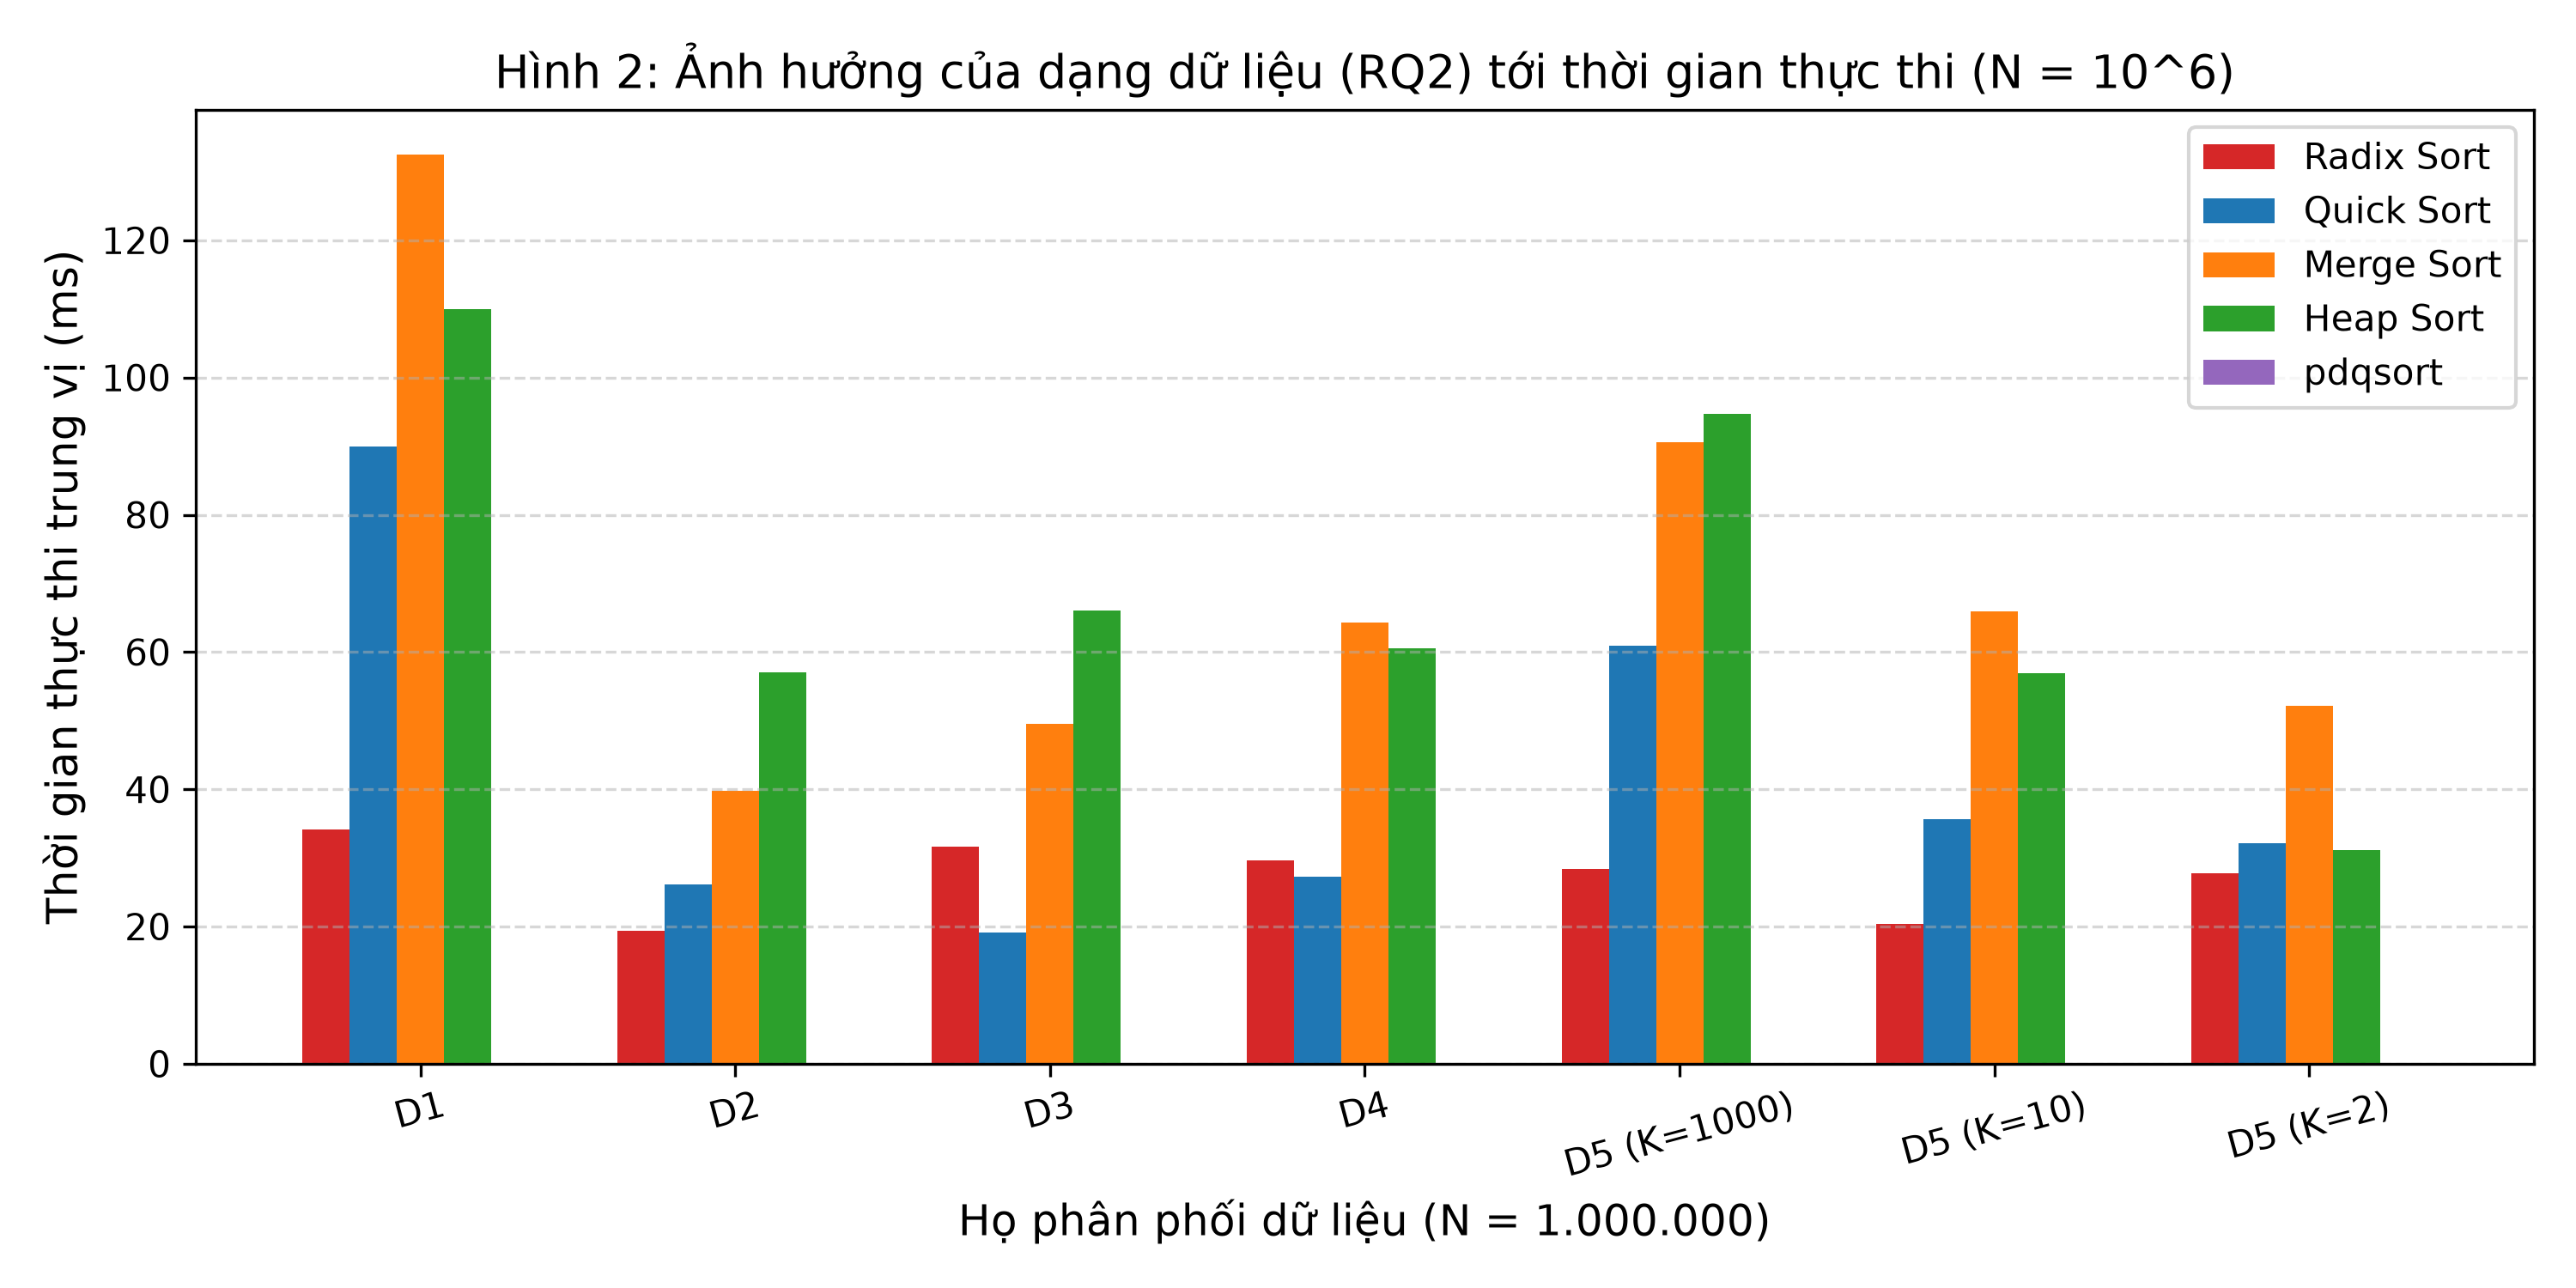
\includegraphics[width=\columnwidth]{fig2_rq2_runtime_by_distribution.png}
\caption{So sánh thời gian thực thi của bốn thuật toán trên các phân phối dữ liệu khác nhau tại $N=10^7$ (RQ2).}
\label{fig:rq2_runtime}
\end{figure}

\begin{figure}[htbp]
\centering
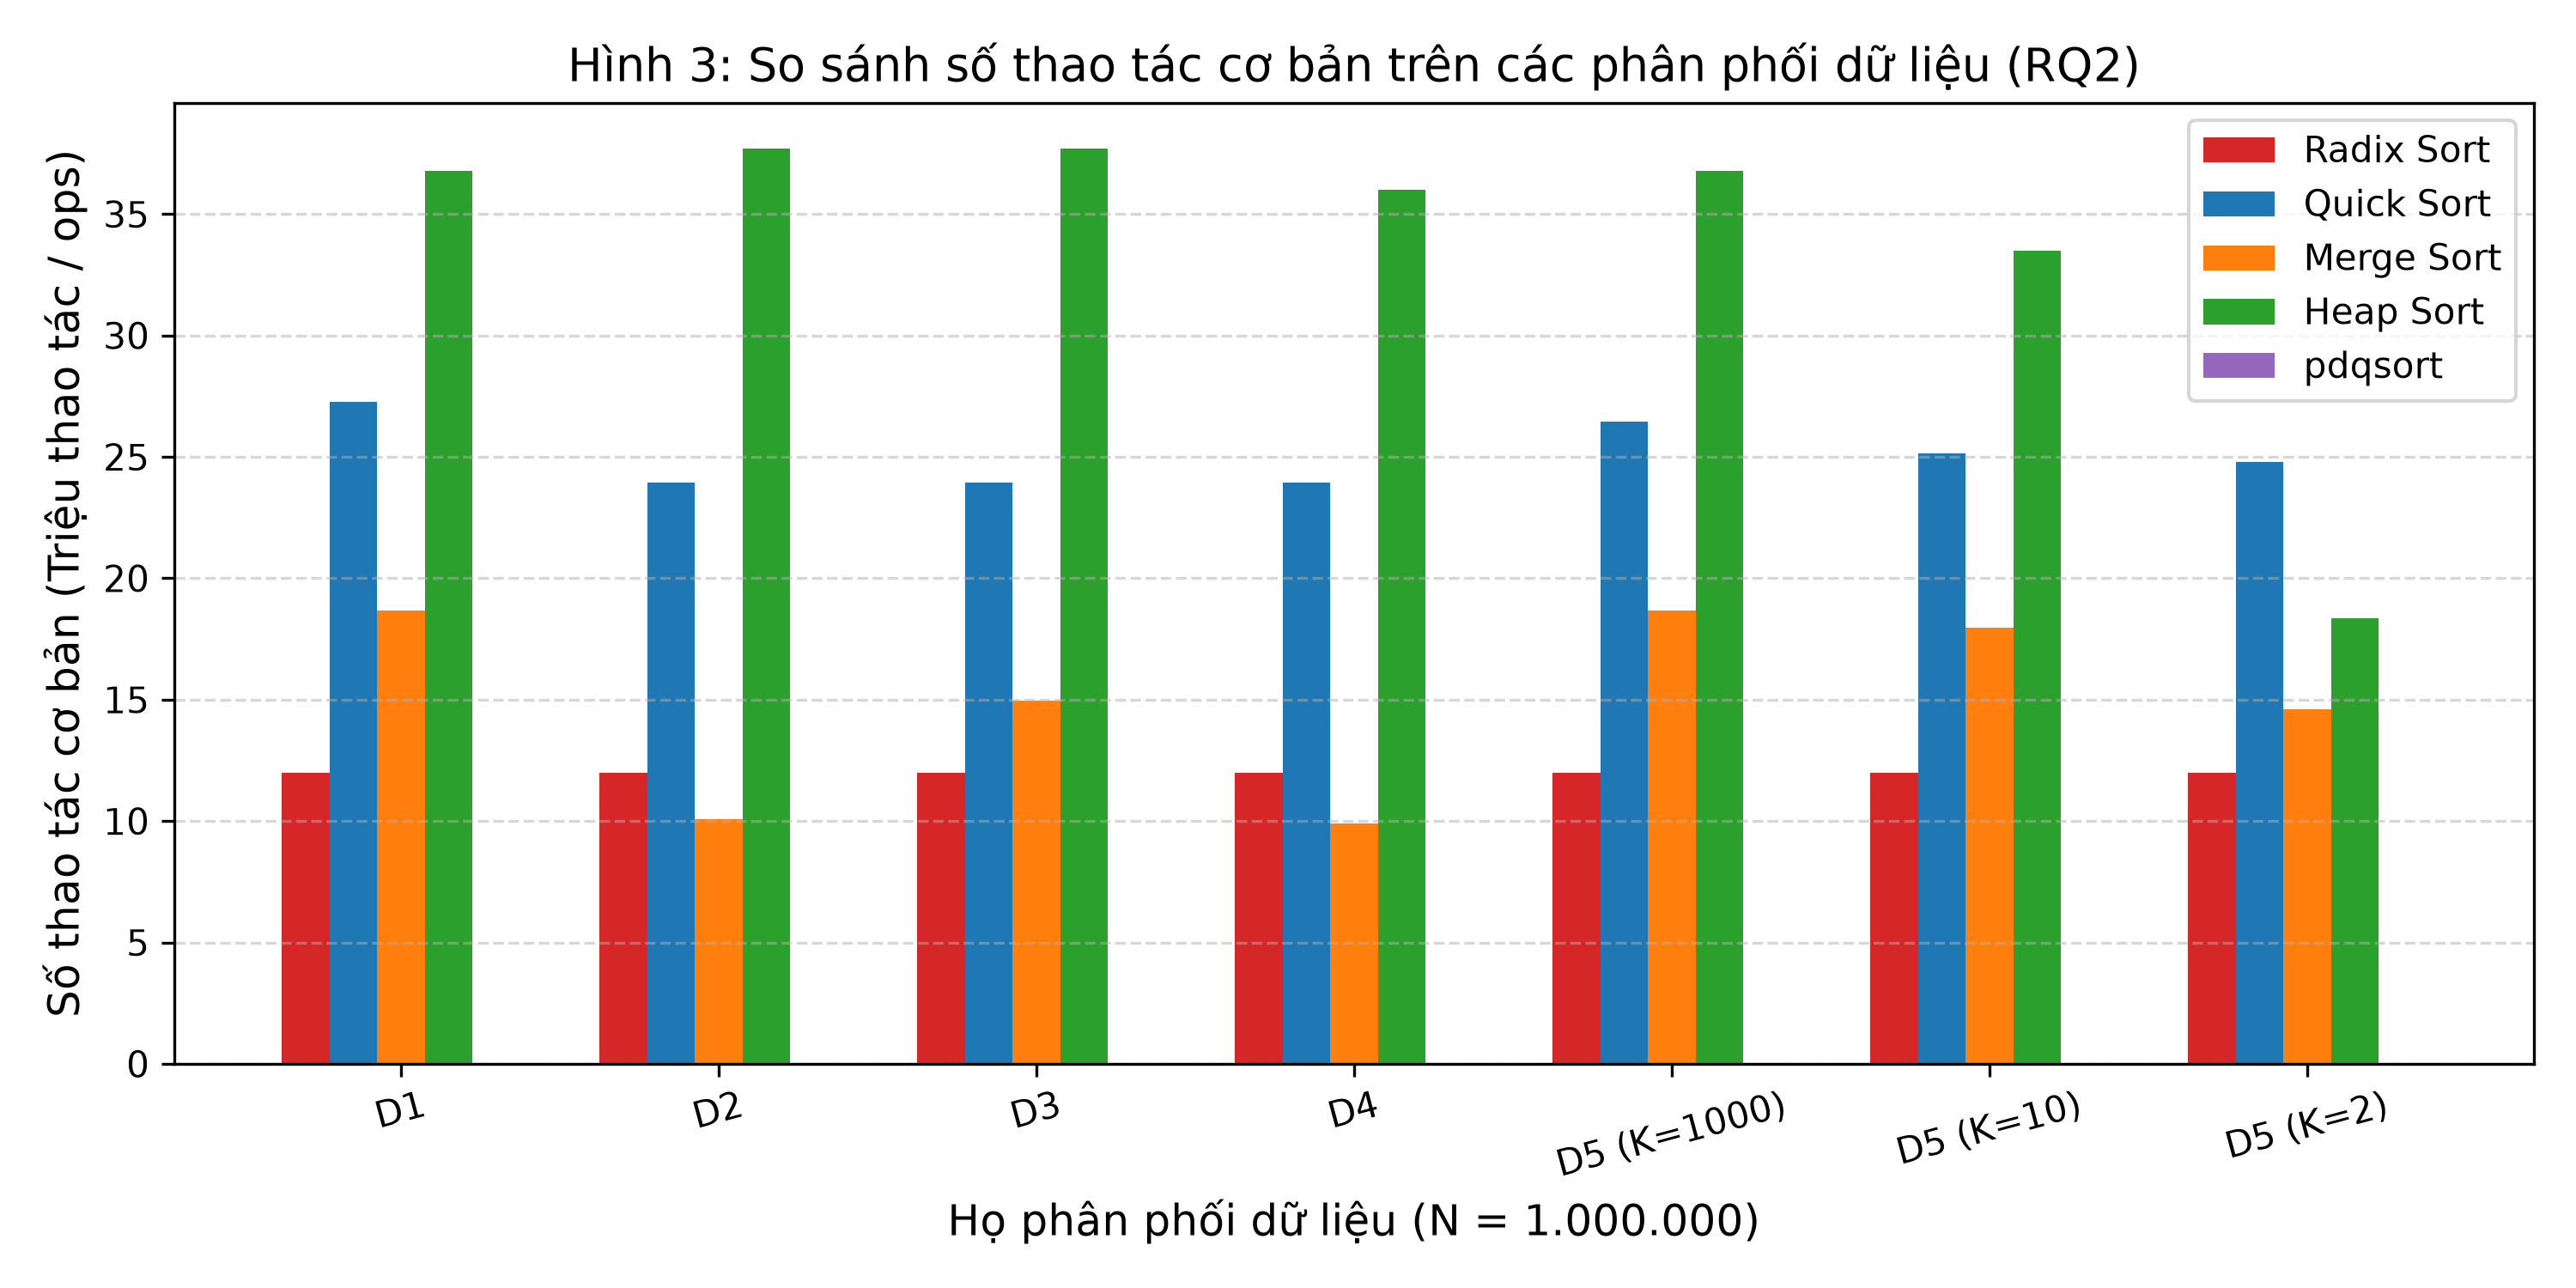
\includegraphics[width=\columnwidth]{fig3_rq2_ops_count.png}
\caption{Số lượng thao tác cơ bản tương ứng của các thuật toán trên các phân phối dữ liệu (RQ2).}
\label{fig:rq2_ops}
\end{figure}

\subsection{RQ3: pdqsort so với Quick Sort và đóng góp của cơ chế A, B}
Bảng~\ref{tab:rq3} báo thời gian (commit \texttt{\RQcommit}); số so sánh lấy từ lượt \texttt{--count} cùng file.

\input{tables/rq3_runtime}

\textbf{pdqsort so với Quick Sort.} Lấy Quick Sort giáo trình làm mốc (cùng $N$, dữ liệu, máy và \texttt{-Xmx}), tỷ lệ median $t_{quick}/t_{pdq}$ là \RQquickOverPdqDone{} trên $D_1$, \RQquickOverPdqDtwo{} trên $D_2$, \RQquickOverPdqDthree{} trên $D_3$, \RQquickOverPdqDfour{} trên $D_4$, \RQquickOverPdqKten{} trên $D_5$ $K=10$ và \RQquickOverPdqKtwo{} trên $D_5$ $K=2$ (Hình~\ref{fig:rq3runtime}).

\textbf{Cơ chế A.} Trên $D_2$, pdqsort đầy đủ tốn \RQpdqOpsPerNDtwo$\,N$ phép so sánh, còn \texttt{noA} tốn \RQnoAOpsPerNDtwo$\,N$: cơ chế A đưa dãy đã sắp về $O(N)$ so sánh. Tại $N=$\RQbigN, tỷ lệ $t_{noA}/t_{pdq}$ là \RQnoAOverPdqDtwo{} trên $D_2$ và \RQnoAOverPdqDfour{} trên $D_4$ (mốc: pdqsort đầy đủ, cùng $N$, dữ liệu, máy).

\textbf{Cơ chế B.} Trên $D_5$ $K=2$, tỷ lệ $t_{noB}/t_{pdq}$ là \RQnoBOverPdqKtwo{} và trên $K=10$ là \RQnoBOverPdqKten{} (mốc: pdqsort đầy đủ, $N=$\RQbigN); số so sánh của \texttt{noB} là \RQnoBOpsPerNKtwo$\,N$ so với \RQpdqOpsPerNKtwo$\,N$ của bản đầy đủ. Không có B, khóa trùng gây phân hoạch lệch liên tục.

\textbf{Kết quả trái dự đoán: JIT che lợi ích của A ở $N$ nhỏ.} Tại $N=$\RQsmallN, $t_{noA}/t_{pdq}$ trên $D_2$ chỉ là \RQnoAOverPdqDtwoSmall{} dù \texttt{noA} tốn gấp \RQnoAOpsOverPdqDtwoSmall{} lần số so sánh. Runner làm nóng trên $D_1$, nơi \texttt{partialInsertionSort} gần như không được gọi, nên lượt đo $D_2$ chạy đường A ở chế độ thông dịch. Gọi lặp 8 lần trong cùng JVM ($D_2$, $N=10^6$, median lần 5--8), bản đầy đủ tốn \RQjitBaseDtwo{} ms, \texttt{noA} tốn \RQjitNoADtwo{} ms (nguồn: \texttt{\RQjitCsv}, \texttt{PdqEvidence jit}).

\begin{figure}[htbp]
\centering
\includegraphics[width=\columnwidth]{fig4_rq3_runtime.png}
\caption{Thời gian median (thanh lỗi min--max, thang log) tại $N = 10^7$. Mục đích: so pdqsort với Quick Sort và thấy cơ chế nào có tác dụng trên dữ liệu nào. Nguồn: \texttt{results/rq3.csv} (\texttt{run\_rq3.ps1}); hình: \texttt{plot\_rq3.py}.}
\label{fig:rq3runtime}
\end{figure}

\begin{figure}[htbp]
\centering
\includegraphics[width=\columnwidth]{fig5_pdq_core_ablation.png}
\caption{Số phép so sánh (thang log) khi tắt từng cơ chế lõi (chưa bật A, B), $N = 10^5$, seed 1. Mục đích: cho thấy mỗi cơ chế lõi đều có tác dụng. Nguồn: \texttt{results/pdq\_ablation.csv} (\texttt{PdqEvidence ablation}); hình: \texttt{plot\_rq3.py}.}
\label{fig:pdqcore}
\end{figure}

\subsection{Khảo sát mảng sát thủ (Killer Adversary Analysis)}
\input{tables/rq3_killer}

Theo Bảng~\ref{tab:killer}, tại $N=10^4$ Quick Sort tốn \RQkillerQuickOpsFour{} phép so sánh (độ sâu \RQkillerQuickDepthFour), pdqsort tốn \RQkillerPdqOpsFour{} (độ sâu \RQkillerPdqDepthFour). Tại $N=10^5$, Quick Sort \texttt{\RQkillerQuickStatusFive} vì StackOverflowError, còn pdqsort \texttt{\RQkillerPdqStatusFive} với độ sâu \RQkillerPdqDepthFive{} nhờ phá mẫu và chuyển sang \texttt{HeapSort.sortRange}.

\section{Đe dọa tính hợp lệ (Threats to Validity)}
\begin{itemize}
    \item \textbf{Tối ưu hóa máy ảo Java (JIT) và GC:} JIT tier-4 compilation có thể làm méo mó kết quả giữa các lần chạy đầu. Nghiên cứu giảm thiểu bằng cách thực hiện 3 lần khởi động (warmup) độc lập và chạy mỗi tiến trình cô lập.
    \item \textbf{Cơ chế quản lý bộ nhớ Heap của OS:} Hàm \texttt{heapBytes} chỉ phản ánh heap pool được quản lý bởi JVM, không đại diện hoàn toàn cho tập làm việc bộ nhớ vật lý (RSS) của tiến trình ở tầng kernel.
    \item \textbf{Giới hạn phạm vi kiểu dữ liệu:} Nghiên cứu tập trung vào khóa số nguyên không âm 32-bit. Các kết luận về Radix Sort có thể thay đổi nếu mở rộng sang khóa 64-bit (\texttt{long}) hoặc số thực dấu phẩy động.
\end{itemize}

\section{Kết luận và Khuyến nghị (Conclusion)}
Qua khảo sát thực nghiệm quy mô lớn trên $10^5 \to 2\times 10^7$ phần tử:
1) \textbf{Radix Sort} là lựa chọn tối ưu tuyệt đối về tốc độ thuần túy cho số nguyên 32-bit nếu hệ thống cho phép dung sai bộ nhớ phụ $O(N)$.
2) \textbf{Heap Sort} là giải pháp bắt buộc trong các hệ thống nhúng hoặc tài nguyên hạn hẹp đòi hỏi bộ nhớ $O(1)$ và bảo đảm không vượt quá $O(N \log N)$.
3) \textbf{pdqsort} chứng minh sự ưu việt toàn diện trong thư viện chuẩn: nó thừa hưởng tốc độ của Quick Sort trên dữ liệu ngẫu nhiên, bứt phá tiệm cận $O(N)$ trên dữ liệu presorted thông qua Cơ chế A, và loại bỏ hoàn toàn suy thoái khóa trùng thông qua Cơ chế B.

\section*{Lời cảm ơn và Khai báo sử dụng AI}
Nhóm nghiên cứu tuyên bố có sử dụng các công cụ trí tuệ nhân tạo (AI Assistant) trong quá trình thực hiện đồ án, bao gồm việc giải thích tài liệu lý thuyết, tối ưu cấu trúc mã nguồn kịch bản benchmark, hỗ trợ định dạng bảng dữ liệu LaTeX theo chuẩn IEEE và rà soát các thuật ngữ chuyên ngành. Mọi số liệu thực nghiệm trong bài báo đều bắt nguồn từ các lượt chạy thực tế trên máy đo, được kiểm chứng chéo toàn diện qua tệp CSV và mã kiểm tra băm đa thức.

\begin{thebibliography}{00}
\bibitem{hoare1962quicksort} C. A. R. Hoare, ``Quicksort,'' \emph{The Computer Journal}, vol. 5, no. 1, pp. 10--16, 1962.
\bibitem{williams1964heapsort} J. W. J. Williams, ``Algorithm 232: Heapsort,'' \emph{Communications of the ACM}, vol. 7, no. 6, pp. 347--348, 1964.
\bibitem{bentley1993engineering} J. L. Bentley and M. D. McIlroy, ``Engineering a sort function,'' \emph{Software: Practice and Experience}, vol. 23, no. 11, pp. 1249--1265, 1993.
\bibitem{peters2021pdqsort} O. R. L. Peters, ``Pattern-defeating quicksort,'' arXiv preprint arXiv:2106.05123, 2021.
\bibitem{musser1997introsort} D. R. Musser, ``Introspective sorting and selection algorithms,'' \emph{Software: Practice and Experience}, vol. 27, no. 8, pp. 983--993, 1997.
\bibitem{mcilroy1999killer} M. D. McIlroy, ``A killer adversary for quicksort,'' \emph{Software: Practice and Experience}, vol. 29, no. 4, pp. 341--344, 1999.
\bibitem{sedgewick2011algorithms} R. Sedgewick and K. Wayne, \emph{Algorithms}, 4th ed. Boston, MA, USA: Addison-Wesley, 2011, \S2.2--2.4, \S5.1.
\end{thebibliography}

\end{document}
